\chapter{Horizon d'exécution étendu et Vol de travail adaptatif}\label{chapter:HX}
%
Dans ce chapitre nous allons présenter les heuristiques proposées pour ordonnancer et placer les threads d'une application décrite par un DAG sur la plateforme NUMA multicoeur. L'\textbf{horizon d'exécution étendu X-VHFU (eXtended Visible, in Horizon, Far and Unseen)} et le \textbf{vol de travail adaptatif basé sur la distance (distance based Work Stealing)} sont les deux idées de base proposées dans cette thèse. 

La première section \ref{schSOP} va exposer l'étude de la combinaison des politiques d'ordo-nnancement et les placements existants appliqués sur des applications constituées d'une séquence de tâches indépendantes. 
Ensuite, nous présentons nos approches dans la deuxième section \ref{OPGT}.
Dans la troisième section \ref{EC}, l'algorithme de l'équilibrage de charge est exposé dont l'heuristique de base est le vol de travail basé sur la distance.
Enfin, la section \ref{conc} conclue le chapitre.
%au premier temps, nous allons les appliquer sur une classe particulière de DAG qui représente les applications parallèles décrites par le modèle de programmation parallèle  fork-join. Ensuite, nous donnons la version généralisée.
%====================================================================================
\section{Schémas des stratégies d'ordonnancement et placement }\label{schSOP}
%
Les algorithmes O/M suivent le même motif structurel, ils diffèrent seulement par la stratégie de la sélection de l'entité courante à être servie. Les schémas algorithmiques suivants explicitent cette idée :

Le schéma pour l'\textbf{ordonnancement des tâches} : il fonctionne selon la stratégie client / serveur en attendant la soumission des tâches à exécuter, il attend la disponibilité d'une ressource d'exécution et puis il choisit la tâche qui optimise une heuristique donnée, enfin il programme l'exécution de celle-ci sur la ressource libérée. Ce schéma est de nature distribuée événementielle selon le motif \textbf{observateur/observable}. L'algorithme \textbf{scheduleTasks} associé avec les évènements \textbf{Event\_OnTaskSubmission} et  \textbf{Event\_-OnTaskExecutionEnd} illustre le principe de ce dernier.

Le schéma pour le \textbf{placement des données} des tâches : il fonctionne selon la stratégie client / serveur en attendant les requêtes des tâches pour charger des données en mémoire ou vers le processeur (deux types de requêtes allocation et libération de la mémoire lecture/écriture des pages/blocs mémoire), il attend la disponibilité d'une ressource de stockage (mémoire) et puis il choisit la requête qui optimise une heuristique donnée, enfin il alloue un espace mémoire dans la mémoire cible pour les données choisies . Ce schéma est aussi de nature distribué évènementiel selon le motif \textbf{observateur/observable}. L'algorithme \textbf{mapTaskData} associé avec les évènements \textbf{Event\_OnTaskAllocateMe-mory}, \textbf{Event\_OnTaskFreeMemory}, \textbf{Event\_OnTaskExecutionStart} et \textbf{Event\_-OnTaskExecutionEnd} illustre le principe de ce dernier.
%-----------------------------------
%\IncMargin{1em}
\begin{algorithm}
\DontPrintSemicolon
\SetNoFillComment % <---------------------------
\SetKwInOut{Input}{input}\SetKwInOut{Output}{output}

%\& $A^* \neq \emptyset$
\Input{A DAG G=(V,E) and a toplogy graph TG=(N,P,L)}
\Output{A schedule of G on TG}

\BlankLine 
\textbf{Function } initialize()\\ 
\Begin{
     \tcc{Q : ready tasks queue , A : available cpus}
	$Q^* \longleftarrow \{T_0\}$ \\
	$A^* \longleftarrow P^*$ \\
	processNotyetScheduledTasks()
}

\BlankLine 

\textbf{Function } processNotyetScheduledTasks()\\ 
\Begin{
	\While { $Q^* \neq \emptyset$} {  
		//ready tasks not executed yet\\
	     \tcc{$T_s$ : selected task to be scheduled now}
		$T_s = $ argMax$_{t \in Q^*}$  TaskSelectionHeuristic($t$)\\
		\If { $T_s \neq \textbf{null}$} { 
			$P_s = $argMax$_{p \in \mathbb{A^*}}$  ProcesseurAllocationHeuristic($p$, $T_s$)\\
			\If { $P_s \neq \textbf{null}$  } {
	     		\tcc{$P_s$ : processor to be allocated now} %				$Q^* = Q^* - \{T_s\}$\\%	$A^* =A^* - \{P_s\}$ 
				Trigger OnTaskExecutionStart($T_s$, $P_s$)\\
				scheduleOn($T_s$, $P_s$).
			}
		}
	}
}

\BlankLine 

\tcc{On task start event}
\textbf{Event }  OnTaskExecutionStart($T$, $P$) \\
\Begin{
	$Q^* = Q^* - \{T_s\}$\\
	$A^* =A^* - \{P\}$ 
}

\tcc{On task end event}
\textbf{Event }  OnTaskExecutionEnd($T$) \\
\Begin{
	$R^*$ = getReadyNeighboursAfterEndOf($T$)\\
	$P$ = getAllocatedProcessorTo($T$)\\
	$Q^* = Q^* \cup R^*$ \\
	$A^* = A^* \cup \{P\}$\\
	processNotyetScheduledTasks()\\
}

\caption{Algorithme générique d'ordonnancement des taches}
\end{algorithm}
%\DecMargin{1em}
%----------------------------------

%-----------------------------------
%\IncMargin{1em}
\begin{algorithm}
\DontPrintSemicolon
\SetNoFillComment % <---------------------------
\SetKwInOut{Input}{input}\SetKwInOut{Output}{output}

%\& $M^* \neq \emptyset$
\Input{A DAG G=(V*,E*) and a toplogy graph TG=(N*[P*,M],L*)}
\Output{A schedule of G on TG}

\BlankLine 

\textbf{Function } initialize()\\ 
\Begin{
     \tcc{$D^*$ : tasks load request data , $M^*$ : available memory pages}
	$D^* \longleftarrow \{T_0.data\}$ \\
	$M^* = getFreeMemoryPages()$ \\
	processnotyetMappedTasksData()
}

\BlankLine 

\textbf{Function } processnotyetMappedTasksData()\\ 
\Begin{
	\While { $D^* \neq \emptyset$} {
	     \tcc{$D^*$ : selected tasks data to be mapped now}
		$S^* = $argMax$_{d \in S^*}$  TaskDataSelectionHeuristic($d$)\\
		\If { $S^* \neq \emptyset$  } {
		     \tcc{$P^*$ : memory pages to be allocated now}
			$D^* = D^* - \{S^*\}$\\
			$P^*_s = $argMax$_{m \in \mathbb{M^*}}$  MemoryMappingHeuristic($m$ , $S^*$)\\
			$M^* =M^* - P^*_s$
		}
	}
}

\BlankLine 

\tcc{On task data load request event}
\textbf{Event }  OnTaskDataLoadRequest($T$,$L^*$) \\
\Begin{
	$D^* = D^* \cup \{L^*\}$\\
	Trigger OnTaskAllocateMemory()
}

\tcc{On task allocate memory event}
\textbf{Event }  OnTaskAllocateMemory() \\
\Begin{
	processnotyetMappedTasksData()
}

\tcc{On task free memory event}
\textbf{Event }  OnTaskFreeMemory($P^*$) \\
\Begin{
	$M^* = M^* \cup \{P^*\}$\\
	processnotyetMappedTasksData()
}

\caption{Algorithme générique de placement des données des taches}
\end{algorithm}
%\DecMargin{1em}
%====================================================================================
\newpage
\section{Ordonnancement et placement des tâches  indépendantes}\label{OPTI}
%
Dans cette section nous allons présenter le cas ou les tâches de l'application sont indépendantes et partagent des données. Dans ce contexte, nous essayons de voir l'impact de la combinaison des différentes politiques d'ordonnancement et de placement sur les performances des applications parallèles. Cela va nous aider à évaluer la  corrélation entre l'ordonnancement et le placement dans le contexte NUMA sans avoir une structure particulière de l'application exécutée. Cette première stratégie nous permet de voir les facteurs influents sur le calcul (exécution) indépendamment de la communication et l'échange des données et d'inspecter le comportement de la plateforme et sa réaction lorsque nous exécutons la même suite de tâches parallèles indépendantes mais en changeant la paire (politique ordonnancement / politique placement) et l'influence de ce fait sur les performances du support exécutif et en particulier le temps total d'exécution, le facteur NUMA et l'équilibrage de charge.
%
\subsection{Combinaison des politiques d'ordonnancement/placement classiques}
Par la suite, nous utilisons certaines politiques implémentées sur les plateformes actuelles pour l'ordonnancement on a :
%
\subsection{Politiques d’ordonnancement classique}
%
\subsubsection{Politique à tour de rôle (Round Robin RRS)} 
%
C'est la politique la plus simple à implémenter elle consiste à allouer les nœuds de calcul aux tâches arrivantes à tour de rôle. Si \textbf{m} est le nombre de nœuds disponibles pour exécution des tâches, et \textbf{(k+1)} est l'ordre d'arrivée de la tâche $T_{k+1}$ (k est le nombre des tâches déjà ordonnancées, cette tâche sera l'entête de la queue \textbf{Q} utilisée pour mettre en file d'attente les tâches reçues. L'heuristique de la sélection des tâches appelle \textbf{Q.pop()} alors cette tâche sera affectée au nœud \textbf{k=n mod m} si ce dernier est libre.
\[
N^*[(k+1) mod |N^*|]
\]
%
\subsubsection{Politique le moins utilisé (LessUsed)}
%
Elle consiste à affecter les tâches arrivantes au nœud le moins utilisé parmi les ressources libres.
\[
		\text{argMin}_{a \in A^*} \text{getProcessorNumberOfUses}(a)
\]
%
\subsubsection{Politique le moins chargé (Less Loaded LLS)}
%
Cette stratégie consiste à surveiller la charge courante de la plateforme en mainte-nant une structure de donnée qui représente sa charge et d'affecter la tâche courante au nœud le moins chargé. L'heuristique de l'allocation détermine argMin des processeurs en fonction de leurs charges obtenues par une fonction getProcessorLoad(p) : 
\[
		\text{argMin}_{a \in A^*} \text{getProcessorsLoad}(a)
\]
%
\subsection{Politiques de placement classique}
%
Nous utilisons des politiques similaires implémentées sur les plateformes actuelles pour le placement et ainsi que d'autre spécifiques au contexte NUMA, on a  :
%
\subsubsection{Placement à tour de rôle (Round Robin RRM)}
%
C'est la politique la plus simple à implémenter elle consiste à allouer les mémoires des nœuds aux tâches à tour de rôle afin de stocker leurs données.
\[
M^*[(k+1) mod |M^*|]
\]
%
\subsubsection{Politique le moins utilisé (LessUsed)}
%
Elle consiste à affecter les tâches arrivantes au nœud le moins utilisé parmi les ressources libres.
\[
		\text{argMin}_{m \in M^*} \text{getMemoryNumberOfUses}(m)
\]
%
\subsubsection{Placement First Touch}
%
Les données d'une tâche seront stockées sur la mémoire du nœud responsable de l'exécution de la tâche associée. Lorsqu’une tâche demande le chargement d'une donnée, le mapper vérifie si elle est déjà chargée dans la mémoire d'un nœud sinon elle sera chargée dans la mémoire du nœud sur lequel la tâche est ordonnancée.%\begin{verbatim}  This is a verbatim block.\end{verbatim}
\[
{\footnotesize
\text{if (T}_i\text{.Load(Data}_j\text{) and Data}_j\text{.State == 'UNLOAD') M[getAllocatedNodeFor(T}_i\text{)].Load(Data}_j\text{)}
}
\]
%
\subsubsection{Placement Next Touch}
%
Les données d'une tâche seront stockées sur la mémoire du nœud responsable de l'exécution de la tâche associée. Lorsqu’une tâche demande le chargement d'une donnée, le mapper verifie si elle est déjà chargée dans la mémoire d'un nœud, alors il va faire migrer cette tâche sinon elle sera chargé dans sa mémoire.%
\[
{\footnotesize
\text{if (T}_i\text{.Load(Data}_j\text{) and Data}_j\text{.State == 'LOAD') M[getAllocatedNodeFor(T}_i\text{)].Migrate(Data}_j\text{)}
}
\]

Les politiques combinées sont round robin RRS, moins utilisé LUS et less loaded LLS pour la stratégie de l'ordonnancement et round robin RRM, moins utilisé LUM, first touch FTM et next-touch NTM pour les stratégies de placement. nous obtenons douze combinaisons.
%====================================================================================
\newpage
\section{Ordonnancement et placement d'un graphe de tâches}\label{OPGT}
%
Dans cette section, nous présentons les idées derrières les heuristiques proposées  ainsi que les algorithmes associés.
%
\subsection{Heuristique Horizon d'exécution Etendu X-VHFU}
%
L'heuristique proposée est constituée de quatre phases. 
Au début de l'exécution, on extrait la \textbf{topologie du DAG} ainsi que les \textbf{informations de communication} (les références et la taille des données utilisées et partagées par les tâches). Cette phase préliminaire est basée sur les annotations faites par le programmeur dans le code source et qui seront convertit à une information utilisée par le support d'exécution. En se basant sur cette topologie on \textbf{partitionne le DAG en sous DAGs} de tailles presque similaire initialement,  
ensuite elle les \textbf{attache aux nœuds} de la plateforme (Fixer les préférences des tâches). 
Lors de l'ordonnancement d'une tâche, en fonction de son horizon d'exécution courant, elle est sélectionnée pour être exécutée soit sur le nœud du sous DAG à lequel cette tâche appartienne ou un autre selon son état courant. Si un autre nœud est choisi alors la configuration des sous DAGs est actualisée en recalculant les nouveaux sous DAG et en appliquant globalement une stratégie dite \textbf{horizon d'exécution X-VHFU} sur le DAG apres ce changement. 
Enfin, elle \textbf{équilibre la charge} en utilisant une stratégie de vol des travaux adapté et basé sur la distance au contexte NUMA.
%
\subsubsection{Partitionner le DAG}
%
Dans cette phase, le DAG $G(V^*,E^*)$ donné est partitionné en $K$ sous DAGs  $(G_i)_{i:1..K}$ en utilisant un algorithme du partitionement des graphes adapté à ce contexte. Dans ce cas , notre graphe sera pondéré avec le volume des donnés échangés entre les tâches (qui peut être obtenu au début l'analyse de notre DAG cible) et non par le temps de la communication entre les tâches (inconnu dans ce contexte). 
Le résultat de cette phase est une partition $G$.   %trouvés dans littérature [@1,@2,@3] 
%
$$
\Phi(G) = (\{ G_1, G_2, \cdots , G_K\}, Mx_{K \times K}) 
$$
$$
G_i = (V^*_i, E^*_i) \text{ vérifiant la relation } \bigcup_{1 \le i \le K} V^*_i = V^* \&  V^*_i \cap V^*_j = \emptyset \text{ , } \forall i \neq j
$$
%
Où $Mx_{K \times K}$ est la matrice de flux inter sous-graphes (volume de données échanger entre les tâches des sous graphes connectés) et $G_i$ le sous graphe numéro $i$. 
Dans un premier temps, notre algorithme doit déterminer les différents niveaux des sommets sur le DAG donné, ensuite il parcourt chaque niveau en essayant d'affecter le sommet courant à un sous graphe qui minimise le flux des données échangées avec le reste des sous graphes déjà calculer.
%----------------------------------%\IncMargin{1em}
\begin{algorithm}
\DontPrintSemicolon
\SetNoFillComment % <---------------------------
\SetKwInOut{Input}{input}\SetKwInOut{Output}{output}

%
\Input{un graphe de tâche DAG G=(V*,E*), La matrice du flux données échangées entre les sommets Md, le nombre des partitions K}
\Output{une partition PAR P = [G*, Mx*], G* l'ensemble des sous DAGs et Mx* : matrice du flux entre les sous DAGs}

\BlankLine 
%\textbf{Function } initialize()\\ 
\Begin{
	L =  getGraphLevels(G)  //Levels\\
	\ForEach{$l \in L$}{
		\ForEach{$v \in l$}{
	$\text{                                                                  }$           j = argMin$_{1 \le i \le K }$ computeEgdeCutWeight(v,G,Md,G*[i],Mx)\\
	$\text{                                                                  }$           G*[j].addVertex(v)\\
	$\text{                                                                  }$           updateEgdeCutWeightMatrix(v,G,Md,G*[j],G,Mx)\\
		}
	}
}

\textbf{Function } getGraphLevels(G(V*,E*))\\ 
\Begin{
	$U = V*$
	$i = 0$\\
	$Levels[i] = $ getVertexWithoutPredecessorsIn(G,U)\\
	\While { $U \neq \emptyset$} {
		$U = U - Levels[i]$\\
		$i++$\\
		$Levels[i] = $ getVertexWithoutPredecessorsIn(G,U)\\
	}
	Return $Levels$
}
\caption{Partitionnement d'un DAG en sous DAGs}
\end{algorithm}              %\DecMargin{1em}
%----------------------------------
Cet algorithme utilise les fonctions helper suivantes :

- \textbf{getGraphLevels(G)} : cette fonction détermine l'ensemble des niveaux des sommets de notre DAG donnée. Comme vu dans le chapitre 2 graphe de tâches, un niveau de rang $l$ dans un DAG est un ensemble de sommets dont les sommets parents sont tous dans le niveau de rang strictement inferieur ou égale à $l-1$ et au moins un sommet parent dans le niveau $l-1$.  le niveau du rang 1 est constitué de l'ensemble des sommets qui n'ont pas de prédécesseurs. La figure \ref{fig:FG_4_1} illustre un DAG avec plusieurs niveaux. 

- \textbf{getVertexWithoutPredecessorsIn(U)} : Cette fonction détermine l'ensemble des sommets qui n'ont pas des sommets prédécesseurs dans l'ensemble $U$. Elle permet de trouver les sommets du niveau courant.

- \textbf{computeEgdeCutWeight(v,G,Md,G*[i],G,Mx)} : cette fonction permet de calculer le flux des données échangés résultant de considérer le sommet $v$ dans le sous graphe $G^*[i]$ en utilisant la matrice des flux trouvée $Mx$. 

- \textbf{updateEgdeCutWeightMatrix(v,G,Md,G*[j],G,Mx)} : cette fonction met à jour la matrice des flux après avoir ajouté $v$ au sous graphe $G^*[j]$.

La figure \ref{fig:FG_4_2} donne un exemple de l'application du processus du partitionnement du DAG donné dans la figure \ref{fig:FG_4_1}. Les sous DAGs résultants sont montrés avec différentes couleurs. 
%
\begin{figure}
\includegraphics[scale=0.6]{dag050}
\centering
\caption{DAG avec plusieurs niveaux}
\label{fig:FG_4_1}
\end{figure}
%
\begin{figure}
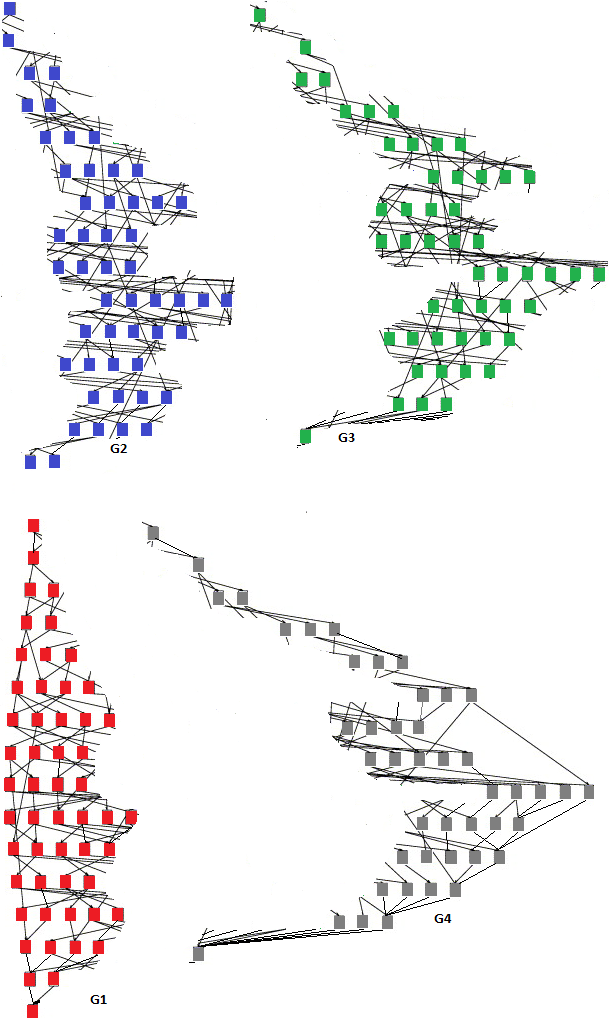
\includegraphics[scale=0.5]{dag053}
\centering
\caption{Resultat de la partition d'un DAG}
\label{fig:FG_4_2}
\end{figure}
%
\subsubsection{Fixer les préférences de tâches en fonction des sous DAGs}
%
Cette deuxième phase consiste à attacher (bind) chaque sous-DAG $G_i$ à un nœud particulier $N_j$ qui sera le nœud espéré d'exécution  des tâches de $G_i$. Cette préférence peut être changée en fonction de l'état actuel du processus généré par l'exécution du DAG $G$.
Cette affectation peut être considérée comme un ordonnancement initial qui  sera actualisé au fur et à mesure qu'on avance dans le processus.
%
$$
\Phi(\{ G_1, G_2, \cdots , G_n\}*, \{N_j\}) = \{(G_{i_1},N_{j_1}), (G_{i_1},N_{j_1}), \cdots, (G_{i_n},N_{j_n}) \}
$$
%----------------------------------%\IncMargin{1em}
\begin{algorithm}
\DontPrintSemicolon
\SetNoFillComment % <---------------------------
\SetKwInOut{Input}{input}\SetKwInOut{Output}{output}

%
\Input{une partition PAR P = [G*, Mx*], matrice des distances NUMA Dx}
\Output{une liste de paires [(G$_i$, N$_j$) i $\in$ I, j $\in$ J] }

\BlankLine 
%\textbf{Function } initialize()\\ 
\Begin{
	Nd* = getAllNode(Dx)\\
	L = $\varnothing$\\
	\ForEach{G$_i$ $\in$ G*}{
%	$\textbf{foreach}$ G$_i$ $\in$ G*\{\\
	$\text{                                                                  }$           N$_j$ = getPreferenceNode(Nd*, G*, G$_i$)\\
	$\text{                                                                  }$           Nd* = Nd* /{N$_i$}\\
	$\text{                                                                  }$           L.addItem((G$_i$,N$_j$))\\
%	$\textbf{endfor}$\\
	}
}

\caption{Préférence d'exécution des sous DAGs}
\end{algorithm}              %\DecMargin{1em}
%----------------------------------
La fonction \textbf{getPreferenceNode(Nd*, G*, G$_i$)} permet de faire une correspondance (bijection, matching) entre les nœuds de la plateforme et les sous DAGs trouvés. Comme le nombre de nœuds $K$ est égal au nombre des sous DAGs alors ce matching revient à trouver une permutation des nœuds dont le nombre est $K!$ qui préserve la relation du voisinage existante entre les sous DAGs en affectant deux sous DAGs voisins sur des nœuds voisin. On peut choisir une métrique qui quantifie une permutation donnée (distance euclidienne ou autre) et ensuite prend le minimum. 
%
\subsubsection{Appliquer la stratégie horizon d'exécution étendu X-VHFU}
%
Lors de l'ordonnancement, la prise de décision de quelle tâche à sélectionner et sur quel nœud doit être exécutée est faite en fonction de l'état actuel du processus correspondant au DAG exécuté. 
%
Apres avoir décidé la tâche à exécuter $T_c$ et le nœud exécutant alors on maintient un partitionnement basé sur la visibilité des tâches au support exécutif. 
Traditionnellement, à un moment donné pendant l'exécution de l'application parallèle décrite par un DAG, l'ensemble des tâches $\mathbb{T}$ est partitionné en quatre catégories :\\
1- Tâches complètes ($C$),  $ T_C$ : Les tâches finies (completed tasks)\\
2- Tâches en exécution $X$, $ T_X$ :  Les tâches en exécution (running tasks)\\
3- Tâches prêtes $R$ (ready task) \\
4- Tâches non prêtes $Q$ (not ready yet task).
%
$$ 
T_R = \{ T \in \mathbb{T} |\forall \text{Parent}(T) \in T_C \}
$$
$$
T_Q = \{ T \in \mathbb{T} | \exists \text{Parent}(T) \notin T_C \}
$$
$$
\mathbb{T} = T_C \cup T_X \cup T_R \cup T_Q
$$
%
Afin de contrôler mieux cette exécution, on partitionne davantage la dernière catégorie $Q$ pour prévoir les tâches visibles à l'instant courant en se basant sur l'information disponible au support exécutif à ce moment (les tâches complètes $C$, les tâche en exécution $X$, tâches prêtes $R$). Cette vision est une extension de la visibilité immédiate à un niveau avancé qui permet d'aller au delà des tâches prêtes $R$. Les nouvelles catégories sont :
%
$$
T_Q = T_V \cup T_H \cup T_F \cup T_U
$$
%
\textbf{Les tâches visibles  $V$ (visible task)}:\\
Les tâches à l'horizon 0, ce sont les tâches qui ont au moins une tâche prédécesseur en exécution et tous autre prédécesseurs sont des tâches  complètes ou en exécution. Apres la terminaison des prédécesseurs qui sont en exécution, Cette tâche change d'état et devient prête. Cette classe de tâche a une forte probabilité d'être exécuté prochainement. 
%
$$
T_V  = \{ T \in \mathbb{T} | \forall \text{Parent}(T) \in T_C \cup T_X \text{ et } \exists \text{Parent}(T) \in T_X \}
$$
% 
\textbf{Les tâches dans l'horizon $H$ (horizon task)} : \\
Les tâches à l'horizon 1, ce sont les tâches qui ont au moins une tâche prédécesseur prête et tous autre prédécesseurs sont des tâches  complètes, en exécution ou prête. On attend que leurs tâches prédécesseurs se terminent avant qu'elles deviennent prêtes. Cette classe de tâche a une probabilité moyenne d'être exécuté prochainement. 
%
$$
T_H  = \{ T \in \mathbb{T} | \forall \text{Parent}(T) \in T_C \cup T_X  \cup T_R  \text{ et } \exists \text{Parent}(T) \in T_R \}
$$
%
\textbf{Les tâches au-delà de l'horizon $F$ (beyond the horizon task)} :\\  %$T_U$ : Les tâches non visibles   \\
Les tâches au-delà de l'horizon non visibles immédiatement qui ont au moins une tâche prédécesseur visible et tous autres prédécesseurs sont des tâches  complètes, en exécution ou visibles. 
%
$$
T_F  = \{ T \in \mathbb{T} | \exists \text{Parent}(T) \notin T_C \cup T_X  \cup T_V  \text{ et } \exists \text{Parent}(T) \in T_V \}\}
$$
%
\textbf{Les tâches non visible $U$ (unseen task)} :\\  %$T_U$ : Les tâches non visibles   \\
Les tâches non visibles sont les tâches qui ont au moins une tâche prédécesseur qui est ni complète, ni en exécutons, ni prête et ni visible. Elles peuvent être loin du niveau actuel de l'exécution. Nous n'avons aucune information qui permet d'évaluer à quel point cette tâche est loin d'être exécutée prochainement. 
%
$$
T_U  = \{ T \in \mathbb{T} | \exists \text{Parent}(T) \notin T_C \cup T_X  \cup T_R  \cup T_V \}
$$
%
Ce partitionnement va nous permettre d'anticiper certaines décisions et de se projeter dans le future prochain de l'exécution de l'application courante. Un nouveau critère de sélection de la tâche courante vient d'être intégré dans le processus de la décision. La prise de décision $D_c$ que l'ordonnanceur doit assurer à chaque libération d'une ressource d'exécution est maintenant une combinaison de trois facteur :
%décision = \Phi(préférence , affinité, horizon) \\
$$
D_c = \Phi(P_f , A_f, H_z) 
$$
%
\textbf{Préférence} $P_f$ : le nœud à lequel le sous DAG qui contient la tâche concernée est attaché.\\
\textbf{Affinité} $A_f$ : le nœud sur lequel une bonne partie des données utilisé par la tâche concernée y résident.\\
\textbf{Horizon} $H_z$ : A quel point si on sélectionne la tâche concernée, on va avancer dans l'horizon d'exécution (on va voir plus de tâches et on s'approche plus de la fin). 

Donc, on partitionne l'ensemble des tâches en fonction de l'horizon d'exécution actuelle (est ce que elle est déjà exécutée ou en court d'exécution, prête, dans l'horizon ou loin d'être exécutés dans le future prochain).
%
\begin{figure}
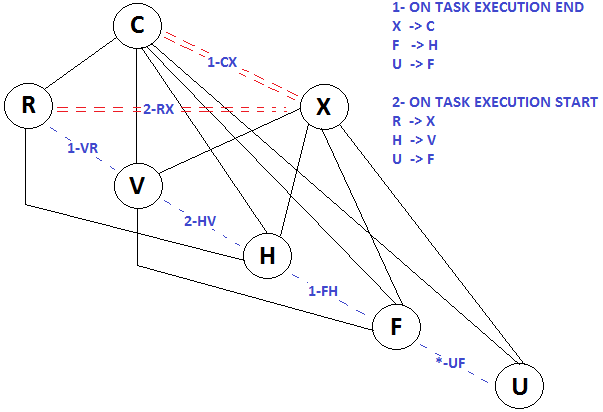
\includegraphics[scale=0.75]{vhfu001}
\centering
\caption{Graphe de transformation des niveaux de visibilité}
\label{fig:FG_4_10}
\end{figure}
%----------------------------------%\IncMargin{1em}
\begin{algorithm}
\DontPrintSemicolon
\SetNoFillComment % <---------------------------
\SetKwInOut{Input}{input}\SetKwInOut{Output}{output}

%
\Input{la tâche récemment terminée ou commencée $T_f$ }
\Output{L'horizon d'exécution courant VHFU}

\BlankLine 
\tcc{On task end event}
\textbf{Event }  OnTaskExecutionEnd($T_e$) \\
\Begin{
	$T_X = T_X - T_e$\\	
	$T_C = T_C \cup {T_e}$\\

     \tcc{update the ready tasks}
	$T_R = T_R \cup $ updateSpecifiedHorizon($T_V$, $T_C$)\\

     \tcc{update the visible tasks}
	$T_H = T_H \cup $  updateSpecifiedHorizon($T_F$, $T_R$)\\

     \tcc{update the visible tasks}
	$T_F = T_F \cup $ updateSpecifiedHorizon($T_U$, $T_V$)\\
}

\BlankLine 
\tcc{On task start event}
\textbf{Event }  OnTaskExecutionStart($T_s$) \\
\Begin{
	$T_R = T_R - T_s$\\	
	$T_X = T_X \cup {T_s}$\\

     \tcc{update the ready tasks}
	$T_V = T_V \cup $ updateSpecifiedHorizon($T_H$, $T_X$)\\

     \tcc{update the visible tasks}
	$T_F = T_F \cup $ updateSpecifiedHorizon($T_U$, $T_V$)\\
}

\tcc{update the specified horizon}
\textbf{Function} updateSpecifiedHorizon($T_A$, $T_B$ )\\
\Begin{
	$V^* = \varnothing$\\
	\ForEach{A$_i$ $\in$ $T_A$}{   %	$\textbf{foreach}$ Q$_i$ $\in$ $Q^*$\\
		\If { $A_i$.getParents() $\subset  T_C \cup T_X  \cup T_B$ and $A_i$.getParents() $\cap T_B \neq \varnothing$  } {
			$V^* = V^* \cup \{ A_i \}$\\
		}
	}
	Return $V^*$
}

\caption{Algorithme Horizon d'exécution étendu XH-VHFU}
\end{algorithm}              %\DecMargin{1em}
%----------------------------------
\begin{figure}
\includegraphics[scale=1]{dag054}
\centering
\caption{DAG avec plusieurs niveaux}
\label{fig:FG_4_1}
\end{figure}

\begin{figure}  %[h]
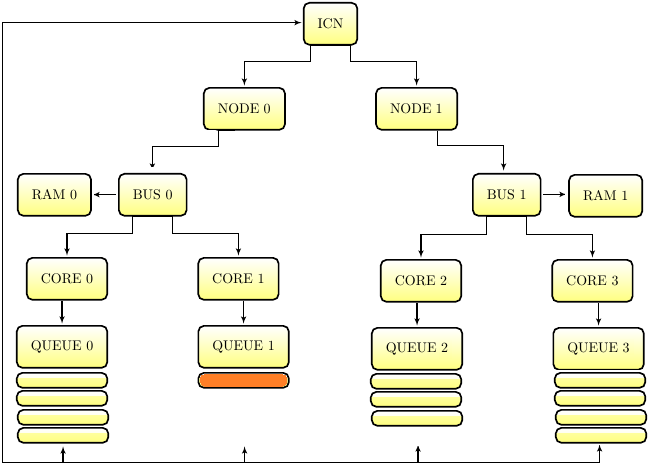
\includegraphics[scale=0.5]{adag003}
\centering
\caption{Plateforme NUMA et stratégie de vol de travail}
\label{fig:hm001}
\end{figure}
%
Le principe de la sélection de la tâche prête à exécuter $T_s$ à un moment donné par l'ordonnanceur est basé sur l'idée de choisir celle qui va élargir l'horizon d'exécution après le changement de son état vers l'exécution pour une meilleure visibilité afin d'avoir plus d'informations qui aident à mieux ordonnancer les tâches suivantes et mieux placer les données associées. Pour déterminer cette tâche $T_s$, l'algorithme parcourt l'ensemble des tâches prêtes $T_R$ et pour chacune d'elle $T_r$ nous allons évaluer la mise à jours de l'horizon de l'exécution $\Delta H(T_r)$ causée par son changement d'état. Cette quantification est une combinaison pondérée du changement de chaque classe de visibilité. De façon intuitive, nous cherchons combien de tâche devient prête $\Delta V(T_r)$, visible $\Delta H(T_r)$, dans horizon $\Delta F(T_r)$ ou au-delà de l'horizon $\Delta U(T_r)$ après avoir choisi d'exécuter la tâche $T_r$. Les classes de visibilité n'ont pas le même degré d'influence ou d'importance sur le processus d'ordonnancement ou placement. La classe visible renseigne ce processus mieux que celle de l'horizon et cette dernière apporte plus d'informations que celle de l'au-delà de l'horizon et en dernier celle l'invisible qui est loin d'être intégrée dans le processus de la prise de décision. Donc, nous allons associer à chaque classe un coefficient ($\alpha, \beta, \gamma, \theta$) comme paramètre de l'importance et l'influence de la mise à jour de la classe courante. Alors la mise à jour globale de l'horizon est fonction linéaire des mises à jour des classes de visibilité pondérées par leurs coefficients.
%
$$
\Delta H^*(T_r) = \alpha \Delta V(T_r) + \beta \Delta H(T_r) + \gamma \Delta F(T_r)  + \theta \Delta U(T_r) 
$$
%
En se basant sur cette formule, nous allons définir nos heuristiques du modèle d'algorithme de l'ordonnancement et placement cités au début de ce chapitre. La première étape consiste définir l'heuristique responsable de la sélection de la tâche à exécuter, ensuite celle qui détermine le nœud à allouer à cette tâche et enfin la stratégie du placement des données.

1- La \textit{tâche prête à choisir} est celle qui va \textbf{élargir au maximum l'horizon d'exécution} $\Delta H(T_r)$.
%
$$
T_s =  \text{argMax}_{T_r \in T_R} \Delta H^*(T_r) 
$$
%
2- Le \textit{nœud à choisir} est celui qui va \textbf{préserver la localité données} ou à \textbf{déjà exécuter les prédécesseurs} de la tâche sélectionnée. Si le nœud du sous DAG contenant cette tâche contient une quantité de donnée utilisée par $T_s$ dont le pourcentage dépasse un seuil prédéfini alors on ne change pas la préférence de $T_s$ et on reste sur le même nœud. Sinon on cherche le nœud qui maximise la localité donnée pour $T_s$.
%
$$
N_s^(T) =
\begin{cases}
SDN(T), & \text{si } getLDx(SDN(T),T) > DL\_THRESHOLD\\
\text{argMax}_{N \in N^*} getLDx(N, T), & \text{sinon}\\
\end{cases}
$$
%
- La fonction \textbf{getLocalityDistance} : permet de calculer pour une tâche $T$ sa distance de localité si elle est affecté au noeud $N$.  \\
- La fonction \textbf{SDN} : subDAGNode permet de déterminer le nœud sur lequel le sous DAG contenant $T_s$ est affecté (préférence).\\
- Le seuil \textbf{DL\_THRESHOLD} : pour décider si on reste sur le nœud de préférence ou on cherche une autre allocation\\
%La fonction \textbf{getDataLocality} : quantifier la localité des données pour la tâche $T_s$ sur le nœud choisi.\\
- La fonction \textbf{getLocalityDistance} : quantifier la localité des données pour la tâche $T_s$ sur le nœud choisi qui est une fonction de la matrice des distances et le placement courant des données de $T_s$ sur la plateforme.\\
3- La mémoire sur laquelle on place les données pendant l'exécution. Pour cette fin, on utilise la stratégie \textbf{Affinity\_on\_first\_Touch} dans sa forme la plus simple sans migration ni modification. c.-à-d. l'allocation de la mémoire pour une requête d'allocation faite par $T_s$ pendant son exécution sera demandée de la mémoire de son nœud. %sur lequel elle s'exécute.
%====================================================================================
\section{Equilibrage de charge}\label{EC}
%
Dans cette phase, un mécanisme classique du vol de travail adapté au contexte NUM qui sera responsable d'équilibrer la charge des entités du support exécutif.
%
\subsection{Vol de travail basé sur distance et adaptatif}
%----------------------------------%\IncMargin{1em}
\begin{algorithm}
\DontPrintSemicolon
\SetNoFillComment % <---------------------------
\SetKwInOut{Input}{input}\SetKwInOut{Output}{output}

%
\Input{\textbf{ICNdx} : Matrix-distance des nœuds NUMA, Paramètres \textbf{Step} : incrément de distance, \textbf{Try} : Nombre de tentative de vols }
\Output{system load balancing state}

\BlankLine 
\Begin{
	\tcc{change the state of the current worker}
	\If {  localTaskQueue.size == THRESHOLD\_MAX\_SIZE } {
		currentWorker.status = VICTIM
	}
	\If {  isEmpty(localTaskQueue) } {
		currentWorker.status = THIEF
	}
	\Else{
	\textbf{run}:    popAtFront(localTaskQueue, task)\\
			execute(task)\\
	\If { localTaskQueue.size == THRESHOLD\_MIN\_SIZE } {
		currentWorker.status = THIEF
	}%          	$\textbf{if}$(localTaskQueue.size == THRESHOLD\_MIN\_SIZE) currentWorker.status = THIEF\\
	}
%	$\textbf{if}$ (localTaskQueue.size == THRESHOLD\_MAX\_SIZE) currentWorker.status = VICTIM\\
%	$\textbf{if}$ (isEmpty(localTaskQueue)) \{\\
%		currentWorker.status = THIEF\\
%	\}\{\\
%	run:    popAtFront(localTaskQueue, task)\\
%			execute(task)\\
%          	$\textbf{if}$(localTaskQueue.size == THRESHOLD\_MIN\_SIZE) currentWorker.status = THIEF\\
%	\} \\
	\If { currentWorker.status == THIEF } {
	dx = Step\\
	theftSuccess = false\\
	count = Try\\
	\While { !theftSuccess and dx < DX\_LIMIT} {%	$\text{while}$ (!theftSuccess and dx < DX\_LIMIT)\{\\
		\For{i =0 to count-1}{                                                         %		$\text{for}$ i =0 to count\{\\
			taskQueue = searchForVictimQueueLessFar(dx, ICNdx) \\
			task = taskQueue.popAtRear()\\
			\If {  !isNull(task) } {
				theftSuccess = true \\
				localTaskQueue.pushAtRear(task)\\
				goto run\\
			}
			\Else{
				\textbf{if } count > 1 \textbf{ then } wait()
			}   %			$\text{if}$( task )\{ \\			\}\{\\							\}\\  %		\}\\
		}
		dx = dx + Step\\   %	\}\\   %		\If { count > 1 } { count = count - 1 }
		\textbf{if } count > 1 \textbf{ then } count = count - 1
	}
}
}
\label{alg:AL_4_3}
\caption{Vol de travail adaptatif basé sur la distance}
\end{algorithm}              %\DecMargin{1em}
%----------------------------------
Algorithme \ref{alg:AL_4_3} vol de travail adaptatif basé sur la distance NUMA a comme entrée les paramètres suivants : \\
\textbf{ICNdx} : La matrice des distances entre les nœuds NUMA. Elle représente les poids associes aux liens du réseau d'interconnexion connectant les nœuds de la plateforme.\\
\textbf{Step} :  C'est un paramètre qui représente l'écart entre les distances successivement  parcourues.\\
\textbf{Try} : Le nombre de tentatives pour passer à une distance supérieure.

Cet algorithme suit la stratégie du vol de travail classique où chaque thread (worker) qui représente un cœur à lequel est associé un ensemble de tâches à exécuter. Chaque worker a une queue associe.\\ 
Les étapes :\\
1- Chaque worker inspecte la taille de sa queue 
si elle est supérieure à $MAX$ alors il change son état à $VICTIM$ en donnant la possibilité aux autres workers de voler des tâches de sa propre queue.
par contre si sa queue est vide alors il passe à état $THIEF$ ou il essaye de voler des tâches des autres workers qui sont dans un état $VICTIM$.
sinon sa queue contient déjà des tâches à exécuter alors il dépile sa queue de l'avant et commence à exécuter la tâche courante et puis il met à jour son état en inspectant la taille de sa queue si elle est passé au dessous de $MIN$ alors il change son état à $THIEF$.

Lors du changement de son état à $THIEF$, le worker lance le processus du vol de travail 
Dans le contexte de $NUMA$ et dans cette variante du vol de travail, l'heuristique conçue est basée sur la matrice distance de NUMA et une distance limite à ne pas dépasser $LIMITE$ car la pénalité de la recherche au-delà de cette distance devient assez importante. 
%et elle pénalise le système fortement
Cette stratégie commence par les nœuds voisins loin par une distance $dx$ spécifiée comme paramètre et si la tentative de vol réussit alors il continue ce processus pour sortir de son état $THIEF$ et revenir à l'état $NORMAL$. Par contre si à un moment donné aucun voisin n'est dans un état de $VICTIM$ alors le worker courant doit voir des nœuds qui sont loin par distance 2dx et il recommence de nouveau la tentative de vol à ce niveau et il continue comme ça jusqu' à ce qu'il revient à son état $NORMAL$ ou il reste sur son état $THIEF$ après avoir fait une tentative de vol et ne trouver aucun $VICTIM$.   

Le code suivant représente le résultat de l'exécution de la commande NUMA sur le système linux  \textbf{numactl --hardware} qui donne la topologie et en particulier la matrice des distances NUMA.
%
\begin{Verbatim}[formatcom=\color{blue}]
// command on NUMA enabled Linux to find out SLIT values provided by BIOS
numactl --hardware

//NUMA SLIT Matrix on 16 Nodes system used for testing - 
node distances:
node   0   1   2   3   4   5   6   7   8   9  10  11  12  13  14  15
  0:  10  13  40  40  62  62  55  55  62  62  55  55  62  62  55  55
  1:  13  10  40  40  62  62  55  55  62  62  55  55  62  62  55  55
  2:  40  40  10  13  55  55  48  48  55  55  48  48  55  55  48  48
  3:  40  40  13  10  55  55  48  48  55  55  48  48  55  55  48  48
  4:  62  62  55  55  10  13  40  40  62  62  55  55  62  62  55  55
  5:  62  62  55  55  13  10  40  40  62  62  55  55  62  62  55  55
  6:  55  55  48  48  40  40  10  13  55  55  48  48  55  55  48  48
  7:  55  55  48  48  40  40  13  10  55  55  48  48  55  55  48  48
  8:  62  62  55  55  62  62  55  55  10  13  40  40  62  62  55  55
  9:  62  62  55  55  62  62  55  55  13  10  40  40  62  62  55  55
 10:  55  55  48  48  55  55  48  48  40  40  10  13  55  55  48  48
 11:  55  55  48  48  55  55  48  48  40  40  13  10  55  55  48  48
 12:  62  62  55  55  62  62  55  55  62  62  55  55  10  13  40  40
 13:  62  62  55  55  62  62  55  55  62  62  55  55  13  10  40  40
 14:  55  55  48  48  55  55  48  48  55  55  48  48  40  40  10  13
 15:  55  55  48  48  55  55  48  48  55  55  48  48  40  40  13  10
\end{Verbatim}

%====================================================================================
\newpage
\section{Conclusion}\label{conc}
%
Dans ce chapitre, nous avons présenté les heuristiques proposées dans cette thèse pour le problème étudié. Alors après une première tentative pour améliorer l'exécution des séquences de tâches indépendantes sur NUMA en combinant les paires des politiques ordonnancement/placement juste pour voir l'impact de cette combinaison sur les perfor-mances de deux processus. Dans un premier temps, nous avons exposé les idées de base de l'heuristique de l'horizon d'exécution étendu pour exécuter les tâches d'un DAG et donné l'algorithme de cette approche. Cette stratégie vise à collecter plus d'informations au processus d'ordonnancement en élargissant l'horizon d'exécution pour avoir une idée des prochaines tâches à exécuter. La décision de l'ordonnancement est basée sur cette métrique en choisissant la tâche qui va élargir le champ de visibilité de notre processus en aidant à mieux explorer le DAG à ordonnancer. 

Ensuite, nous avons présenté la deuxième approche le vol de travail basé sur la distance qui est une adaptation de la stratégie du vol de travail conçu pour les multicores et variante pour la plateforme NUMA dont le but d'équilibrer la charge des nœuds. Cette stratégie tient en compte l'information collectée au début sur la plateforme (extraction de la topologie de l'environnement d'exécution et sa matrice de distance). Elle vise à limiter le champ du vol à une certaine distance, un certain nombre de fois si cela ne réussit pas alors elle va augmenter cette distance et voir. Par ce principe, elle favorise les nœuds qui sont proches et elle évite les nœuds ou la pénalité NUMA est importante (en fonction de la distance entre les deux nœuds concernés).
 
Le chapitre suivant constitue le cadre général pour expérimenter (en simulant), évaluer et tester l'apport des ces heuristiques dans le contexte de NUMA pour le problème étudié.